\documentclass[10pt,aspectratio=169]{beamer}

% Compile with XeLaTeX
\usepackage{fontspec}
\setsansfont{Arial}
\setmainfont{Times New Roman}
\usepackage{amsmath,booktabs,array,tabularx}
\usepackage{tikz}
\usetikzlibrary{arrows.meta,positioning,calc,fit,shapes.geometric,decorations.pathreplacing}
\usepackage{hyperref}

% ---------- Visual system ----------
\definecolor{navy}{HTML}{F7F5F0}
\definecolor{panel}{HTML}{FFFFFF}
\definecolor{paneltwo}{HTML}{E8F0F1}
\definecolor{cyan}{HTML}{007C83}
\definecolor{blue}{HTML}{2855A6}
\definecolor{orange}{HTML}{B86418}
\definecolor{green}{HTML}{14775A}
\definecolor{red}{HTML}{D53F4F}
\definecolor{ink}{HTML}{17283A}
\definecolor{muted}{HTML}{607080}
\definecolor{paper}{HTML}{FFFFFF}

\setbeamercolor{normal text}{fg=ink,bg=navy}
\setbeamercolor{frametitle}{fg=ink,bg=navy}
\setbeamercolor{structure}{fg=cyan}
\setbeamercolor{alerted text}{fg=orange}
\setbeamerfont{frametitle}{family=\rmfamily,series=\bfseries,size=\Large}
\setbeamerfont{title}{family=\rmfamily,series=\bfseries,size=\Huge}
\setbeamertemplate{navigation symbols}{}
\setbeamertemplate{itemize item}{\color{cyan}$\blacktriangleright$}
\setbeamertemplate{itemize subitem}{\color{orange}$\bullet$}
\setlength{\leftmargini}{1.3em}

% Academic light background: paper tone, rule, dot grid and circuit watermark.
\setbeamertemplate{background}{%
\begin{tikzpicture}[remember picture,overlay]
  \fill[navy] (current page.south west) rectangle (current page.north east);
  \fill[cyan!6] ($(current page.north east)+(-.20,0)$) rectangle (current page.south east);
  \fill[cyan] ($(current page.north west)+(.32,-.34)$) rectangle ++(.12,-.48);
  \draw[cyan!55,line width=.8pt] ($(current page.north west)+(.55,-.83)$) -- ($(current page.north east)+(-.55,-.83)$);
  \draw[ink!10,line width=.35pt] ($(current page.north west)+(.55,-.88)$) -- ($(current page.north east)+(-.55,-.88)$);
  \begin{scope}[shift={(current page.north east)}]
    \foreach \x in {0,...,4}{\foreach \y in {0,...,7}{
      \fill[cyan!25] ({-.36-.16*\x},{-1.18-.16*\y}) circle (.5pt);
    }}
    \draw[cyan!17,line width=.55pt] (-.45,-3.0)--(-1.05,-3.0)--(-1.35,-3.3)--(-2.05,-3.3);
    \fill[cyan!25] (-1.35,-3.3) circle (1.4pt);
    \draw[cyan!17,line width=.55pt] (-.45,-3.45)--(-.9,-3.45)--(-1.2,-3.75)--(-1.85,-3.75);
  \end{scope}
  \node[anchor=south east,text=cyan!7,font=\rmfamily\bfseries\fontsize{46}{48}\selectfont]
    at ($(current page.south east)+(-.6,.82)$) {SPI};
\end{tikzpicture}}

\setbeamercolor{author in head/foot}{bg=paper,fg=muted}
\setbeamercolor{date in head/foot}{bg=paper,fg=ink}

\newcommand{\slideno}{\insertframenumber/22}
\setbeamertemplate{footline}{%
  \pgfmathsetlengthmacro{\progresswidth}{\paperwidth*\insertframenumber/22}%
  \begin{beamercolorbox}[wd=\paperwidth,ht=.7pt,dp=0pt]{author in head/foot}%
    \color{paneltwo}\rule{\paperwidth}{.7pt}\hspace{-\paperwidth}\color{cyan}\rule{\progresswidth}{.7pt}%
  \end{beamercolorbox}%
  \leavevmode\hbox{%
  \begin{beamercolorbox}[wd=.78\paperwidth,ht=3.1ex,dp=1.25ex,leftskip=.55cm]{author in head/foot}%
    \color{muted}\scriptsize SPI — Serial Peripheral Interface
  \end{beamercolorbox}%
  \begin{beamercolorbox}[wd=.22\paperwidth,ht=3.1ex,dp=1.25ex,rightskip=.55cm plus1fil]{date in head/foot}%
    \hfill\color{ink}\scriptsize\bfseries \slideno
  \end{beamercolorbox}}}

\newcommand{\source}[1]{\par\vspace{.3ex}{\tiny\color{muted}Nguồn: #1}}
\newcommand{\pill}[2]{\tikz[baseline=(n.base)]\node[rounded corners=3pt,fill=#1!10,draw=#1!75,inner xsep=6pt,inner ysep=2.5pt,text=#1,font=\scriptsize\bfseries](n){#2};}
\newcommand{\metric}[3]{%
  \begin{tikzpicture}[baseline]
    \node[rounded corners=3pt,fill=panel,draw=#1!55,line width=.7pt,minimum width=2.48cm,minimum height=1.18cm,align=center] {
      {\color{#1}\bfseries\large #2}\\[-1pt]{\color{muted}\scriptsize #3}};
  \end{tikzpicture}}
\newenvironment{darkbox}[1][cyan]{\begin{beamercolorbox}[rounded=true,sep=7pt,wd=\linewidth]{block body}\color{ink}}{\end{beamercolorbox}}
\setbeamercolor{block body}{bg=panel,fg=ink}
\setbeamercolor{block title}{bg=paneltwo,fg=cyan}

\tikzset{
  device/.style={rounded corners=4pt,draw=cyan!70,fill=panel,line width=1pt,minimum width=3.15cm,minimum height=2.2cm,align=center,text=ink},
  smallchip/.style={rounded corners=3pt,draw=blue!65,fill=panel,line width=.7pt,minimum width=1.75cm,minimum height=.82cm,align=center,text=ink,font=\scriptsize\bfseries},
  sig/.style={-Latex,very thick},
  bit/.style={draw=cyan!65,fill=paneltwo,minimum width=.44cm,minimum height=.48cm,font=\scriptsize\bfseries,text=ink},
  note/.style={rounded corners=3pt,fill=orange!8,draw=orange!65,text=ink,align=center,font=\scriptsize}
}

\title{SPI — Serial Peripheral Interface}
\subtitle{Fundamentals \& Working Principles}
\author{Mạnh — Đạt — Phúc}
\institute{Môn học: Vi xử lí – Vi điều khiển}
\date{Tháng 10/2026}

\begin{document}

% ========================= 1 =========================
\begin{frame}[plain]
\transfade[duration=.35]
\begin{tikzpicture}[remember picture,overlay]
  \fill[navy] (current page.south west) rectangle (current page.north east);
  \fill[cyan!8] (current page.north east) -- ++(-6.3,0) -- ++(6.3,-5.0) -- cycle;
  \foreach \y in {-2.4,-1.7,...,2.5}{
    \draw[cyan!22,line width=.7pt] ($(current page.east)+(0,\y)$) -- ++(-1.2,0) -- ++(-.45,.45) -- ++(-1.1,0);
  }
  \node[draw=cyan!75,fill=panel,very thick,rounded corners=10pt,minimum width=3.3cm,minimum height=3.3cm] (chip) at ($(current page.east)+(-3.15,0.55)$) {};
  \node[text=cyan,font=\bfseries\fontsize{27}{29}\selectfont] at (chip) {SPI};
  \foreach \i in {-1.2,-.4,.4,1.2}{
    \draw[cyan!75,line width=2pt] ($(chip.west)+(0,\i)$)--++(-.48,0);
    \draw[cyan!75,line width=2pt] ($(chip.east)+(0,\i)$)--++(.48,0);
  }
  \node[font=\tiny,text=muted,anchor=north] at ($(chip.south)+(0,-.15)$) {SCLK · MOSI · MISO · CS};
\end{tikzpicture}

\vspace{.55cm}
{\color{cyan}\bfseries\large SERIAL COMMUNICATION / 01}\par
\vspace{.28cm}
{\rmfamily\fontsize{29}{32}\selectfont\bfseries SPI — Serial\\Peripheral Interface}\par
\vspace{.28cm}
{\Large\color{muted}Fundamentals \& Working Principles}\par
\vspace{.55cm}
\pill{cyan}{Serial}\hspace{.3em}\pill{blue}{Synchronous}\hspace{.3em}\pill{orange}{Full-duplex}
\vfill
{\color{ink}\bfseries Mạnh — Đạt — Phúc}\hspace{.6em}{\color{muted}| Vi xử lí – Vi điều khiển}\par
\vspace{.38cm}

\begin{tikzpicture}
 \foreach \x/\t/\c in {0/Fundamentals/cyan,3.35/Timing \& Implementation/blue,7.3/Applications \& Debug/orange}{
   \fill[\c] (\x,0) rectangle ++(2.95,.08);
   \node[anchor=north west,text=\c,font=\scriptsize\bfseries] at (\x,-.08) {\t};
 }
\end{tikzpicture}
\begin{tikzpicture}[remember picture,overlay]
  \fill[cyan!5] ($(current page.north east)+(-5.7,-1.0)$) -- ($(current page.north east)+(0,-1.0)$) -- ($(current page.north east)+(0,-7.5)$) -- cycle;
  \node[draw=cyan!75,fill=panel,line width=1.3pt,rounded corners=5pt,minimum width=3.15cm,minimum height=3.15cm] (coverchip) at ($(current page.east)+(-3.0,.65)$) {};
  \node[text=cyan,font=\rmfamily\bfseries\fontsize{27}{29}\selectfont] at (coverchip) {SPI};
  \foreach \i in {-1.15,-.38,.38,1.15}{
    \draw[cyan!75,line width=1.4pt] ($(coverchip.west)+(0,\i)$)--++(-.45,0);
    \draw[cyan!75,line width=1.4pt] ($(coverchip.east)+(0,\i)$)--++(.45,0);
  }
  \draw[blue!28,line width=.7pt] ($(coverchip.east)+(.45,1.15)$)--++(.55,0)--++(.3,.3)--++(.8,0);
  \draw[orange!30,line width=.7pt] ($(coverchip.east)+(.45,-.38)$)--++(.8,0)--++(.35,-.35)--++(.55,0);
  \node[font=\tiny,text=muted,anchor=north] at ($(coverchip.south)+(0,-.18)$) {SCLK · MOSI · MISO · CS};
\end{tikzpicture}
\end{frame}

% ========================= 2 =========================
\begin{frame}{Overview of Serial Communication}
\transwipe[direction=0,duration=.35]
\vspace{-.25cm}
\begin{columns}[T,onlytextwidth]
\column{.49\textwidth}
{\color{muted}\scriptsize 01 — CÁCH DỮ LIỆU DI CHUYỂN}\par\vspace{.2cm}
\begin{tikzpicture}[x=1cm,y=1cm]
  \node[smallchip,minimum width=1.45cm] (a) at (0,1.5) {TX};
  \node[smallchip,minimum width=1.45cm] (b) at (4.1,1.5) {RX};
  \foreach \y in {.85,1.03,...,2.1} {\draw[-Latex,muted!65,line width=.45pt] (.78,\y)--(3.32,\y);}
  \node[text=ink,font=\bfseries] at (2.05,2.48) {PARALLEL};
  \node[text=muted,font=\scriptsize,align=center] at (2.05,.45) {N bit cùng lúc · nhiều chân\\dễ skew / crosstalk};
  \node[smallchip,minimum width=1.45cm] (c) at (0,-.9) {TX};
  \node[smallchip,minimum width=1.45cm] (d) at (4.1,-.9) {RX};
  \draw[-Latex,cyan,line width=2pt] (.78,-.9)--(3.32,-.9);
  \foreach \x/\v in {1.05/1,1.42/0,1.79/1,2.16/0,2.53/0,2.90/1}{\node[text=cyan,font=\tiny\bfseries] at (\x,-.63) {\v};}
  \node[text=ink,font=\bfseries] at (2.05,-.05) {SERIAL};
  \node[text=muted,font=\scriptsize,align=center] at (2.05,-1.78) {từng bit · ít chân\\dễ đi dây PCB};
\end{tikzpicture}

\column{.49\textwidth}
{\color{muted}\scriptsize 02 — CÁCH HAI BÊN CANH THỜI GIAN}\par\vspace{.25cm}
\begin{beamercolorbox}[rounded=true,sep=8pt]{block body}
\textbf{Synchronous}\hfill\pill{cyan}{SPI · I²C}\par\vspace{.25cm}
{\small Có đường clock riêng; dữ liệu được lấy mẫu theo cạnh clock.}
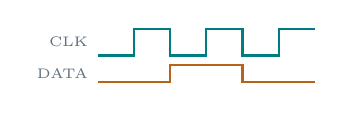
\begin{tikzpicture}[x=.46cm,y=.34cm]
  \draw[cyan,thick] (0,0)--(1,0)--(1,1)--(2,1)--(2,0)--(3,0)--(3,1)--(4,1)--(4,0)--(5,0)--(5,1)--(6,1);
  \draw[orange,thick] (0,-1)--(2,-1)--(2,-.35)--(4,-.35)--(4,-1)--(6,-1);
  \node[anchor=east,text=muted,font=\tiny] at (0,.5){CLK};
  \node[anchor=east,text=muted,font=\tiny] at (0,-.7){DATA};
\end{tikzpicture}
\end{beamercolorbox}
\vspace{.25cm}
\begin{beamercolorbox}[rounded=true,sep=8pt]{block body}
\textbf{Asynchronous}\hfill\pill{orange}{UART}\par\vspace{.25cm}
{\small Không có clock chung; hai bên thống nhất baud rate, dùng start/stop bit.}
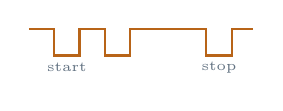
\begin{tikzpicture}[x=.46cm,y=.34cm]
  \draw[orange,thick] (0,1)--(.7,1)--(.7,0)--(1.4,0)--(1.4,1)--(2.1,1)--(2.1,0)--(2.8,0)--(2.8,1)--(4.9,1)--(4.9,0)--(5.6,0)--(5.6,1)--(6.2,1);
  \node[text=muted,font=\tiny] at (1.05,-.45){start}; \node[text=muted,font=\tiny] at (5.25,-.45){stop};
\end{tikzpicture}
\end{beamercolorbox}
\end{columns}
\vfill
\begin{center}\pill{cyan}{SPI = SERIAL + SYNCHRONOUS}\end{center}
\end{frame}

% ========================= 3 =========================
\begin{frame}{What is SPI?}
\transfade[duration=.35]
\begin{columns}[T,onlytextwidth]
\column{.55\textwidth}
\vspace{.25cm}
{\color{cyan}\fontsize{20}{22}\selectfont\bfseries Serial Peripheral Interface}\par
\vspace{.18cm}{\color{muted}Một bus nối tiếp đồng bộ, chuẩn \textit{de facto}, dành cho giao tiếp cự ly ngắn giữa các IC.}\par
\vspace{.5cm}
\begin{tikzpicture}[node distance=.5cm and .5cm]
 \node[smallchip,draw=cyan,minimum width=3.05cm,minimum height=1.05cm] (s) {SERIAL\\[-2pt]\color{muted}\tiny từng bit};
 \node[smallchip,draw=blue,right=of s,minimum width=3.05cm,minimum height=1.05cm] (y) {SYNCHRONOUS\\[-2pt]\color{muted}\tiny có SCLK};
 \node[smallchip,draw=orange,below=of s,minimum width=3.05cm,minimum height=1.05cm] (f) {FULL-DUPLEX\\[-2pt]\color{muted}\tiny gửi + nhận đồng thời};
 \node[smallchip,draw=green,right=of f,minimum width=3.05cm,minimum height=1.05cm] (s) {CONTROLLER–PERIPHERAL\\[-2pt]\color{muted}\tiny một bên tạo clock};
\end{tikzpicture}

\column{.41\textwidth}
\begin{beamercolorbox}[rounded=true,sep=10pt]{block body}
{\color{orange}\bfseries Không có “một chuẩn SPI duy nhất”}\par\vspace{.25cm}
{\small Mode, độ dài frame, thứ tự bit và giao thức lệnh phụ thuộc từng IC.}\par\vspace{.35cm}
\pill{orange}{LUÔN ĐỌC DATASHEET}
\end{beamercolorbox}
\vspace{.4cm}
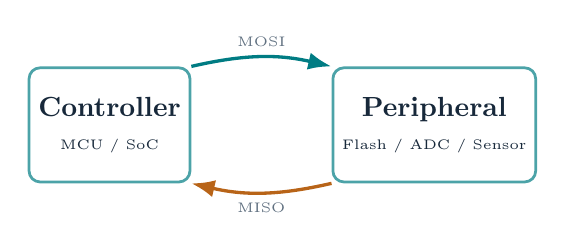
\begin{tikzpicture}
 \node[device,minimum width=1.9cm,minimum height=1.45cm] (c) {\bfseries Controller\\\tiny MCU / SoC};
 \node[device,minimum width=1.9cm,minimum height=1.45cm,right=1.78cm of c] (p) {\bfseries Peripheral\\\tiny Flash / ADC / Sensor};
 \draw[-Latex,cyan,very thick,bend left=13] (c.north east) to node[above,text=muted,font=\tiny]{MOSI} (p.north west);
 \draw[-Latex,orange,very thick,bend left=13] (p.south west) to node[below,text=muted,font=\tiny]{MISO} (c.south east);
\end{tikzpicture}
\end{columns}
\vfill
\source{\href{https://www.analog.com/en/resources/analog-dialogue/articles/introduction-to-spi-interface.html}{Analog Devices — Introduction to SPI}; \href{https://docs.kernel.org/spi/spi-summary.html}{Linux Kernel — SPI summary}.}
\end{frame}

% ========================= 4 =========================
\begin{frame}{SPI Architecture}
\transwipe[direction=90,duration=.35]
\vspace{-.15cm}
\begin{center}
\begin{tikzpicture}[x=1cm,y=1cm]
 \node[device,minimum width=3.25cm,minimum height=3.7cm] (c) at (0,0) {};
 \node[text=cyan,font=\bfseries\large] at ($(c.north)+(0,-.5)$) {CONTROLLER};
 \node[smallchip,minimum width=2.1cm] at ($(c.center)+(0,.35)$) {Clock Generator};
 \node[smallchip,minimum width=2.1cm] at ($(c.center)+(0,-.72)$) {Shift Register};
 \node[device,minimum width=3.25cm,minimum height=3.7cm,draw=orange!75] (p) at (8.8,0) {};
 \node[text=orange,font=\bfseries\large] at ($(p.north)+(0,-.5)$) {PERIPHERAL};
 \node[smallchip,minimum width=2.1cm,draw=orange!65] at ($(p.center)+(0,.35)$) {Control Logic};
 \node[smallchip,minimum width=2.1cm,draw=orange!65] at ($(p.center)+(0,-.72)$) {Shift Register};

 \draw[sig,cyan] ($(c.east)+(0,1.1)$)--node[above,text=ink,font=\bfseries\scriptsize]{SCLK} node[below,text=muted,font=\tiny]{controller phát clock} ($(p.west)+(0,1.1)$);
 \draw[sig,blue] ($(c.east)+(0,.34)$)--node[above,text=ink,font=\bfseries\scriptsize]{MOSI} ($(p.west)+(0,.34)$);
 \draw[sig,orange] ($(p.west)+(0,-.42)$)--node[above,text=ink,font=\bfseries\scriptsize]{MISO} ($(c.east)+(0,-.42)$);
 \draw[sig,green] ($(c.east)+(0,-1.15)$)--node[above,text=ink,font=\bfseries\scriptsize]{$\overline{\mathrm{CS}}$} node[below,text=muted,font=\tiny]{active-low} ($(p.west)+(0,-1.15)$);
 \draw[muted,line width=1.5pt] ($(c.south)+(0,-.45)$)--node[below,text=muted,font=\scriptsize]{GND chung — mốc tham chiếu điện áp} ($(p.south)+(0,-.45)$);
 \node[note] at (4.4,2.18) {\textbf{4 tín hiệu logic} + GND chung};
\end{tikzpicture}
\end{center}
\vspace{.15cm}
\begin{columns}[onlytextwidth]
\column{.32\textwidth}\metric{cyan}{SCLK}{clock → peripheral}
\column{.32\textwidth}\metric{blue}{MOSI}{data → peripheral}
\column{.32\textwidth}\metric{orange}{MISO}{data → controller}
\end{columns}
\vfill
\source{Analog Devices, \href{https://www.analog.com/en/resources/reference-designs/circuits-from-the-lab/cn0564.html}{CN0564 — SPI signaling summary}.}
\end{frame}

% ========================= 5 =========================
\begin{frame}{SPI Signal Lines}
\transfade[duration=.35]
\vspace{-.15cm}
\begin{columns}[T,onlytextwidth]
\column{.63\textwidth}
\scriptsize
\renewcommand{\arraystretch}{1.22}
\begin{tabularx}{\linewidth}{>{\bfseries}l >{\color{muted}}l X}
\toprule
\color{ink}Tín hiệu & \color{ink}Hướng & \color{ink}Vai trò \\
\midrule
\color{cyan}SCLK & Controller $\rightarrow$ Peripheral & Clock đồng bộ; mỗi chu kỳ dịch một bit \\
\color{blue}MOSI / COPI & Controller $\rightarrow$ Peripheral & Dữ liệu controller gửi đi \\
\color{orange}MISO / CIPO & Peripheral $\rightarrow$ Controller & Dữ liệu peripheral gửi về \\
\color{green}$\overline{\mathrm{CS}}$ / SS / NSS & Controller $\rightarrow$ Peripheral & Chọn chip; thường kích hoạt mức thấp \\
\bottomrule
\end{tabularx}
\vspace{.35cm}
\begin{beamercolorbox}[rounded=true,sep=7pt]{block body}
\pill{orange}{MẸO ĐẤU NỐI}\hspace{.35em}{\small Nối theo \textbf{hướng tín hiệu}, không nối theo chữ giống nhau.}\par\vspace{.2cm}
{\small SDI/DIN của peripheral $\leftarrow$ \textbf{MOSI}; \quad SDO/DOUT $\rightarrow$ \textbf{MISO}.}
\end{beamercolorbox}

\column{.33\textwidth}
\begin{tikzpicture}[x=.56cm,y=.43cm]
 \node[smallchip,minimum width=1.4cm,minimum height=3.85cm] (c) at (0,0) {CTRL};
 \node[smallchip,minimum width=1.4cm,minimum height=3.85cm,draw=orange] (p) at (5,0) {PERI};
 \draw[sig,cyan] (.8,1.5)--node[above,text=cyan,font=\bfseries\tiny]{SCLK}(4.2,1.5);
 \draw[sig,blue] (.8,.5)--node[above,text=blue,font=\bfseries\tiny]{MOSI}(4.2,.5);
 \draw[sig,orange] (4.2,-.5)--node[above,text=orange,font=\bfseries\tiny]{MISO}(.8,-.5);
 \draw[sig,green] (.8,-1.5)--node[above,text=green,font=\bfseries\tiny]{$\overline{CS}$}(4.2,-1.5);
 \node[note,minimum width=2.8cm] at (2.5,-2.75) {CS$\downarrow$: bắt đầu\\CS$\uparrow$: kết thúc};
\end{tikzpicture}
\end{columns}
\vfill
\source{\href{https://www.analog.com/en/resources/app-notes/an-1248.html}{Analog Devices AN-1248 — SPI Interface}.}
\end{frame}

% ========================= 6 =========================
\begin{frame}{Single and Multiple Peripheral Connections}
\transwipe[direction=0,duration=.35]
\vspace{-.15cm}
\begin{columns}[T,onlytextwidth]
\column{.62\textwidth}
{\color{cyan}\bfseries PHỔ BIẾN — BUS CHUNG, CS RIÊNG}\par\vspace{.18cm}
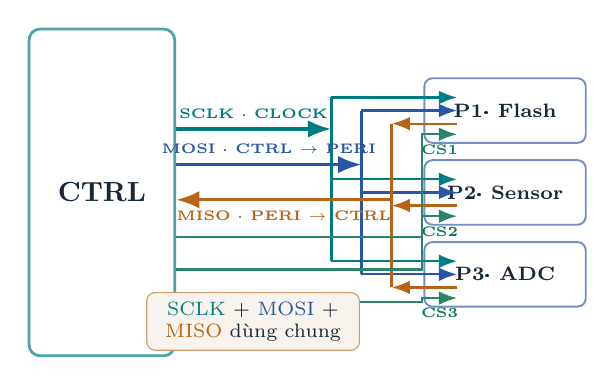
\begin{tikzpicture}[x=.64cm,y=.52cm]
 \node[device,minimum width=1.85cm,minimum height=4.15cm] (c) at (0,0) {\bfseries CTRL};
 \foreach \y/\n/\lab in {2/1/Flash,0/2/Sensor,-2/3/ADC}{
   \node[smallchip,minimum width=2.05cm] (p\n) at (8,\y) {P\n · \lab};
 }

 % Ba đường bus dùng chung, mỗi đường có nhãn ngay tại đoạn xuất phát.
 \draw[cyan,very thick,-Latex] ($(c.east)+(0,1.55)$)--node[above,text=cyan,font=\tiny\bfseries]{SCLK · CLOCK} (4.55,1.55);
 \draw[cyan,very thick] (4.55,2.32)--(4.55,-1.68);
 \foreach \y in {2,0,-2}{\draw[cyan,thick,-Latex] (4.55,{\y+.32})--(7.05,{\y+.32});}

 \draw[blue,very thick,-Latex] ($(c.east)+(0,.68)$)--node[above,text=blue,font=\tiny\bfseries]{MOSI · CTRL $\rightarrow$ PERI} (5.15,.68);
 \draw[blue,very thick] (5.15,2.0)--(5.15,-2.0);
 \foreach \y in {2,0,-2}{\draw[blue,thick,-Latex] (5.15,\y)--(7.05,\y);}

 \draw[orange,very thick,-Latex] (5.75,-.18)--node[below,text=orange,font=\tiny\bfseries]{MISO · PERI $\rightarrow$ CTRL} ($(c.east)+(0,-.18)$);
 \draw[orange,very thick] (5.75,1.68)--(5.75,-2.32);
 \foreach \y in {2,0,-2}{\draw[orange,thick,-Latex] (7.05,{\y-.32})--(5.75,{\y-.32});}

 % Mỗi peripheral có một chân CS riêng.
 \foreach \y/\n/\start in {2/1/-1.08,0/2/-1.88,-2/3/-2.68}{
   \draw[green!90,thick,-Latex] ($(c.east)+(0,\start)$) -| (6.35,{\y-.58}) -- node[below,text=green,font=\tiny\bfseries]{CS\n} (7.05,{\y-.58});
 }
 \node[note,text width=2.45cm,minimum width=2.7cm] at (3.0,-3.15) {\textcolor{cyan}{SCLK} + \textcolor{blue}{MOSI} + \textcolor{orange}{MISO} dùng chung};
\end{tikzpicture}
\vspace{.08cm}
\begin{center}\pill{cyan}{TỔNG SỐ DÂY = 3 + N}\end{center}

\column{.35\textwidth}
\begin{beamercolorbox}[rounded=true,sep=8pt]{block body}
{\color{orange}\bfseries Quy tắc MISO}\par\vspace{.25cm}
{\small Peripheral không được chọn phải nhả MISO về \textbf{high-Z}. Hai chip cùng lái đường này $\Rightarrow$ bus contention.}
\end{beamercolorbox}
\vspace{.28cm}
{\color{cyan}\bfseries DAISY-CHAIN}\par\vspace{.2cm}
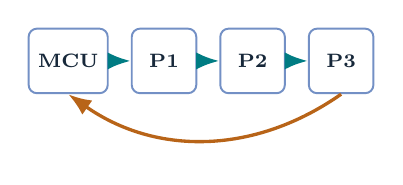
\begin{tikzpicture}[node distance=.28cm]
 \node[smallchip,minimum width=1.0cm] (m) {MCU};
 \node[smallchip,minimum width=.82cm,right=of m] (a) {P1};
 \node[smallchip,minimum width=.82cm,right=of a] (b) {P2};
 \node[smallchip,minimum width=.82cm,right=of b] (d) {P3};
 \draw[sig,cyan] (m)--(a); \draw[sig,cyan] (a)--(b); \draw[sig,cyan] (b)--(d);
 \draw[sig,orange,bend left=35] (d.south) to (m.south);
\end{tikzpicture}
{\small\color{muted}Một CS chung; tiết kiệm chân nhưng tăng độ trễ và mọi thiết bị phải hỗ trợ.}
\end{columns}
\vfill
\source{\href{https://www.analog.com/en/resources/analog-dialogue/articles/introduction-to-spi-interface.html}{Analog Devices — Multi-subnode SPI}.}
\end{frame}

% ========================= 7 =========================
\begin{frame}{Internal SPI Hardware Architecture}
\transfade[duration=.35]
\vspace{-.15cm}
\begin{center}
\begin{tikzpicture}[x=1cm,y=1cm]
 \node[smallchip,minimum width=1.65cm,minimum height=1.25cm,draw=green] (cpu) at (0,0) {CPU / DMA};
 \node[smallchip,minimum width=1.55cm] (tx) at (2.25,.9) {TX FIFO};
 \node[smallchip,minimum width=1.55cm] (rx) at (2.25,-.9) {RX FIFO};
 \node[smallchip,minimum width=2.05cm,minimum height=1.45cm] (sr1) at (4.75,0) {SHIFT REGISTER\\\color{muted}\tiny controller · 8/16 bit};
 \node[smallchip,minimum width=2.05cm,minimum height=1.45cm,draw=orange] (sr2) at (9.65,0) {SHIFT REGISTER\\\color{muted}\tiny peripheral};
 \node[smallchip,minimum width=2.25cm,draw=orange] (ctl) at (4.75,2.0) {CONTROL LOGIC\\\color{muted}\tiny mode · order · flags};
 \node[smallchip,minimum width=2.15cm,draw=cyan] (clk) at (7.15,-2.0) {CLOCK GENERATOR\\\color{muted}\tiny prescaler};

 \draw[sig,green] (cpu.north east)--node[above,text=muted,font=\tiny]{ghi} (tx.west);
 \draw[sig,green] (rx.west)--node[below,text=muted,font=\tiny]{đọc} (cpu.south east);
 \draw[sig,blue] (tx.east)--(sr1.north west);
 \draw[sig,orange] (sr1.south west)--(rx.east);
 \draw[sig,blue] (sr1.east)--node[above,text=blue,font=\scriptsize\bfseries]{MOSI · bit đi} (sr2.west);
 \draw[sig,orange,bend left=18] (sr2.south west) to node[below,text=orange,font=\scriptsize\bfseries]{MISO · bit về} (sr1.south east);
 \draw[muted,thick,-Latex] (ctl.south)--node[right,text=muted,font=\tiny]{điều khiển} (sr1.north);
 \draw[cyan,very thick] (clk.east)--node[below,text=cyan,font=\scriptsize\bfseries]{SCLK} (sr2.south |- clk.east);
 \draw[sig,cyan] (sr2.south |- clk.east)--(sr2.south);
 \node[note,minimum width=3.0cm] at (7.2,1.45) {MOSI + MISO tạo\\\textbf{vòng dịch hai chiều}};
\end{tikzpicture}
\end{center}
\vspace{.25cm}
\begin{columns}[onlytextwidth]
\column{.24\textwidth}\metric{green}{TX / RX}{đệm CPU hoặc DMA}
\column{.24\textwidth}\metric{blue}{SHIFT}{dịch từng bit}
\column{.24\textwidth}\metric{cyan}{$f_{SCLK}$}{$f_{PCLK}$/prescaler*}
\column{.24\textwidth}\metric{orange}{CONTROL}{mode · CS · flags}
\end{columns}
\vfill
\source{Sơ đồ khái quát; chi tiết tùy MCU. Microchip, \href{https://developerhelp.microchip.com/xwiki/bin/view/products/mcu-mpu/32bit-mcu/sam/samd21-mcu-overview/peripherals/sercom-spi-master/}{SAM D21 SERCOM SPI overview}.}
\end{frame}

% ========================= 8 =========================
\begin{frame}{How SPI Transfers Data}
\transglitter[direction=90,duration=.4]
\vspace{-.18cm}
\begin{columns}[T,onlytextwidth]
\column{.48\textwidth}
{\color{cyan}\bfseries MỖI CLOCK = 1 BIT GỬI + 1 BIT NHẬN}\par\vspace{.22cm}
\begin{tikzpicture}[x=.49cm,y=.55cm]
 \node[text=muted,font=\scriptsize,anchor=east] at (-.3,.5){CTRL};
 \foreach \x/\v in {0/1,1/0,2/1,3/0,4/0,5/1,6/0,7/1}{\node[bit] at (\x,.5){\v};}
 \node[text=blue,font=\scriptsize\bfseries,anchor=west] at (8,.5){0xA5};
 \node[text=muted,font=\scriptsize,anchor=east] at (-.3,-1){PERI};
 \foreach \x/\v in {0/0,1/0,2/1,3/1,4/1,5/1,6/0,7/0}{\node[bit,draw=orange!75] at (\x,-1){\v};}
 \node[text=orange,font=\scriptsize\bfseries,anchor=west] at (8,-1){0x3C};
 \draw[sig,blue] (1,-.05)--node[above,text=blue,font=\tiny]{MOSI}(6,-.05);
 \draw[sig,orange] (6,-.45)--node[below,text=orange,font=\tiny]{MISO}(1,-.45);
 \draw[decorate,decoration={brace,mirror,amplitude=5pt},cyan] (-.3,-1.55)--(7.3,-1.55) node[midway,below=.15cm,text=ink,font=\scriptsize]{8 xung $\Rightarrow$ hoán đổi 1 frame};
\end{tikzpicture}
\vspace{.55cm}
\begin{beamercolorbox}[rounded=true,sep=8pt]{block body}
{\small\textbf{MSB-first} (phổ biến) hoặc \textbf{LSB-first} (tùy thiết bị).}\par\vspace{.2cm}
{\small Sau 8 xung: controller nhận \textcolor{orange}{\textbf{0x3C}}, peripheral nhận \textcolor{blue}{\textbf{0xA5}}.}
\end{beamercolorbox}

\column{.49\textwidth}
{\color{muted}\scriptsize MINH HỌA MODE 0 · GIÁ TRỊ TỰ ĐẶT}\par\vspace{.15cm}
\begin{tikzpicture}[x=.35cm,y=.47cm]
 \node[anchor=east,text=muted,font=\tiny] at (0,2.5){SCLK};
 \draw[cyan,thick] (0,2)--(1,2);
 \foreach \x in {1,3,...,15}{\draw[cyan,thick] (\x,2)--(\x,3)--(\x+1,3)--(\x+1,2);}
 \draw[cyan,thick] (16,2)--(17,2);
 \node[anchor=east,text=muted,font=\tiny] at (0,.9){MOSI};
 \foreach \i/\v in {0/1,1/0,2/1,3/0,4/0,5/1,6/0,7/1}{
   \draw[blue,thick] ({1+2*\i},{.45+.9*\v})--({3+2*\i},{.45+.9*\v});
   \node[text=blue,font=\tiny\bfseries] at ({2+2*\i},{.9+.9*\v}){\v};
 }
 \node[anchor=east,text=muted,font=\tiny] at (0,-.75){MISO};
 \foreach \i/\v in {0/0,1/0,2/1,3/1,4/1,5/1,6/0,7/0}{
   \draw[orange,thick] ({1+2*\i},{-1.2+.9*\v})--({3+2*\i},{-1.2+.9*\v});
   \node[text=orange,font=\tiny\bfseries] at ({2+2*\i},{-.75+.9*\v}){\v};
 }
 \foreach \x in {1,3,...,15}{\draw[green!75,dashed,thin] (\x,-1.45)--(\x,3.25);}
 \node[note,minimum width=4.55cm] at (8,-2.1) {Muốn \textbf{đọc} vẫn phải phát clock\\$\Rightarrow$ controller gửi dummy byte};
\end{tikzpicture}
\end{columns}
\vfill
\source{\href{https://docs.kernel.org/spi/spi-summary.html}{Linux Kernel — SPI shifting}; \href{https://www.analog.com/en/resources/analog-dialogue/articles/introduction-to-spi-interface.html}{Analog Devices — data transmission}.}
\end{frame}

% ========================= 9 =========================
\begin{frame}{SPI Transaction Structure}
\transwipe[direction=180,duration=.35]
\vspace{-.15cm}
\begin{center}
\begin{tikzpicture}[x=.73cm,y=.55cm]
 \node[anchor=east,text=muted,font=\scriptsize] at (0,2.3){$\overline{CS}$};
 \draw[green,very thick] (0,2.8)--(1,2.8)--(1,1.8)--(14.5,1.8)--(14.5,2.8)--(15.5,2.8);
 \draw[green!65,dashed] (1,1.55)--(1,-1.25); \draw[green!65,dashed] (14.5,1.55)--(14.5,-1.25);
 \node[text=green,font=\scriptsize\bfseries] at (1,3.25){START};
 \node[text=green,font=\scriptsize\bfseries] at (14.5,3.25){END / LATCH};
 \fill[blue!70] (1,.15) rectangle (4,1.25);
 \fill[cyan!65] (4,.15) rectangle (7.2,1.25);
 \fill[orange!75] (7.2,.15) rectangle (9.6,1.25);
 \fill[green!65] (9.6,.15) rectangle (14.5,1.25);
 \node[text=ink,font=\bfseries] at (2.5,.7){COMMAND};
 \node[text=ink,font=\bfseries] at (5.6,.7){ADDRESS};
 \node[text=ink,font=\bfseries] at (8.4,.7){DUMMY};
 \node[text=ink,font=\bfseries] at (12.05,.7){DATA ···};
 \draw[decorate,decoration={brace,mirror,amplitude=6pt},cyan] (1,-.1)--(4,-.1) node[midway,below=.25cm,text=muted,font=\scriptsize]{1 frame = 8 bit (thường gặp)};
 \draw[decorate,decoration={brace,mirror,amplitude=8pt},orange] (1,-1.15)--(14.5,-1.15) node[midway,below=.28cm,text=ink,font=\bfseries\scriptsize]{1 transaction = toàn bộ thời gian CS ở mức active};
\end{tikzpicture}
\end{center}
\vspace{.25cm}
\begin{columns}[T,onlytextwidth]
\column{.24\textwidth}
\textcolor{blue}{\bfseries COMMAND}\par{\small\color{muted}Đọc, ghi, xóa hoặc opcode.}
\column{.24\textwidth}
\textcolor{cyan}{\bfseries ADDRESS}\par{\small\color{muted}Thanh ghi / ô nhớ đích.}
\column{.24\textwidth}
\textcolor{orange}{\bfseries DUMMY}\par{\small\color{muted}Clock chờ nếu IC yêu cầu.}
\column{.24\textwidth}
\textcolor{green}{\bfseries DATA}\par{\small\color{muted}Một hoặc nhiều byte.}
\end{columns}
\vspace{.1cm}
\begin{beamercolorbox}[rounded=true,sep=7pt]{block body}
\small\textcolor{orange}{\bfseries Không phải khuôn cố định:} định dạng lệnh và yêu cầu giữ/nhả CS do \textbf{datasheet của peripheral} quyết định.
\end{beamercolorbox}
\vfill
\source{Linux Kernel, \href{https://docs.kernel.org/spi/spi-summary.html}{SPI summary}; cấu trúc transaction là mô hình khái quát.}
\end{frame}

% ========================= 10 =========================
\begin{frame}{SPI Read and Write Operations}
\transfade[duration=.35]
\vspace{-.2cm}
\begin{columns}[T,onlytextwidth]
\column{.49\textwidth}
\begin{beamercolorbox}[rounded=true,sep=6pt]{block body}
\pill{blue}{WRITE}\hfill{\color{muted}\scriptsize MISO: thường bỏ qua}\par\vspace{.18cm}

\begin{tikzpicture}[x=.65cm,y=.6cm]
 \fill[blue!45] (0,0) rectangle (3,1); \node[text=ink,font=\bfseries\scriptsize] at (1.5,.5){WRITE CMD / ADDR};
 \fill[green!42] (3,0) rectangle (6,1); \node[text=ink,font=\bfseries\scriptsize] at (4.5,.5){DATA};
 \draw[green,thick] (-.35,1.35)--(0,1.35)--(0,1.12)--(6,1.12)--(6,1.35)--(6.35,1.35);
 \node[text=muted,font=\tiny,anchor=east] at (-.4,1.28){CS};
\end{tikzpicture}
{\small CS$\downarrow$ $\rightarrow$ lệnh/địa chỉ $\rightarrow$ dữ liệu $\rightarrow$ CS$\uparrow$}
\end{beamercolorbox}
\vspace{.15cm}
\begin{beamercolorbox}[rounded=true,sep=6pt]{block body}
\pill{orange}{READ}\hfill{\color{muted}\scriptsize MOSI tạo clock}\par\vspace{.18cm}
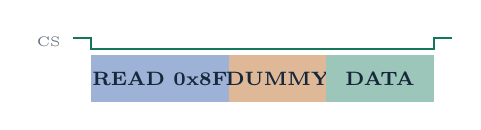
\begin{tikzpicture}[x=.65cm,y=.6cm]
 \fill[blue!45] (0,0) rectangle (2.7,1); \node[text=ink,font=\bfseries\scriptsize] at (1.35,.5){READ 0x8F};
 \fill[orange!45] (2.7,0) rectangle (4.6,1); \node[text=ink,font=\bfseries\scriptsize] at (3.65,.5){DUMMY};
 \fill[green!42] (4.6,0) rectangle (6.7,1); \node[text=ink,font=\bfseries\scriptsize] at (5.65,.5){DATA};
 \draw[green,thick] (-.35,1.35)--(0,1.35)--(0,1.12)--(6.7,1.12)--(6.7,1.35)--(7.05,1.35);
 \node[text=muted,font=\tiny,anchor=east] at (-.4,1.28){CS};
\end{tikzpicture}
{\small Gửi \textbf{dummy 0x00} để tạo 8 clock; dữ liệu thực đi về trên MISO.}
\end{beamercolorbox}

\column{.47\textwidth}
{\color{cyan}\bfseries TẠI SAO CẦN DUMMY?}\par\vspace{.2cm}
{\small SPI chỉ dịch bit khi SCLK chạy. Muốn nhận 8 bit, controller vẫn phải phát 8 xung — thường bằng cách gửi một byte không quan tâm.}
\vspace{.2cm}
\begin{beamercolorbox}[rounded=true,sep=6pt]{block body}
{\color{green}\bfseries BURST TRANSFER}\par\vspace{.3cm}
\begin{tikzpicture}[x=.55cm,y=.55cm]
 \fill[blue!45] (0,0) rectangle (1.8,.8); \node[text=ink,font=\tiny\bfseries] at (.9,.4){CMD};
 \foreach \x/\n in {1.8/0,3.1/1,4.4/2,5.7/3}{\fill[green!42] (\x,0) rectangle ++(1.25,.8);\node[text=ink,font=\tiny\bfseries] at (\x+.625,.4){D\n};}
 \draw[decorate,decoration={brace,mirror,amplitude=5pt},orange] (0,-.12)--(6.95,-.12) node[midway,below=.2cm,text=muted,font=\tiny]{giữ CS thấp · địa chỉ thường tự tăng};
\end{tikzpicture}
{\small Một lệnh, nhiều byte $\Rightarrow$ giảm overhead so với nhiều transaction rời.}
\end{beamercolorbox}
\vspace{.15cm}
\begin{beamercolorbox}[rounded=true,sep=5pt]{block body}
{\scriptsize\color{muted}Ví dụ \textbf{0x8F} chỉ để minh họa quy ước bit 7 = READ; không đại diện cho mọi IC.}
\end{beamercolorbox}
\end{columns}
\vfill
\source{\href{https://www.analog.com/en/resources/technical-articles/add-usb-to-anything.html}{Analog Devices — SPI command/data}; opcode và dummy cycle theo datasheet.}
\end{frame}

% ========================= 11 =========================
\begin{frame}{SPI vs I²C, UART and CAN}
\transwipe[direction=90,duration=.4]
\vspace{-.22cm}
\scriptsize
\renewcommand{\arraystretch}{.96}
\setlength{\tabcolsep}{3.2pt}
\begin{tabularx}{\linewidth}{>{\color{muted}\bfseries}l >{\color{cyan}\centering\arraybackslash}X >{\centering\arraybackslash}X >{\centering\arraybackslash}X >{\centering\arraybackslash}X}
\toprule
 & \textcolor{cyan}{\bfseries SPI} & \textbf{I²C} & \textbf{UART} & \textbf{CAN} \\
\midrule
Clock & SCLK riêng & SCL riêng & không có & clock recovery \\
Dây & $3+N$ & 2 & 2 & 2 vi sai \\
Hướng & full-duplex & half-duplex & full-duplex & half-duplex \\
Chọn node & CS riêng & địa chỉ & point-to-point & ID + arbitration \\
Tin cậy & không ACK/CRC & ACK & parity tùy chọn & ACK + CRC \\
Tốc độ & \textbf{vài–chục MHz*} & 0.1–3.4 Mbit/s & kbps–vài Mbps* & 1 Mbit/s cổ điển* \\
Phù hợp & flash, ADC, LCD & sensor, RTC & console, module & ô tô, công nghiệp \\
\bottomrule
\end{tabularx}
\vspace{.28cm}
\begin{columns}[T,onlytextwidth]
\column{.58\textwidth}
\begin{beamercolorbox}[rounded=true,sep=7pt]{block body}
{\color{cyan}\bfseries CHỌN SPI KHI}\quad
{\small cần \textbf{tốc độ cao}, overhead thấp, full-duplex, khoảng cách ngắn và số peripheral vừa phải.}
\end{beamercolorbox}
\vspace{.18cm}
{\scriptsize\color{muted}* Tốc độ SPI/UART phụ thuộc IC và PCB. CAN FD cho phép pha dữ liệu nhanh hơn; bảng giữ mốc Classical CAN để dễ so sánh.}

\column{.39\textwidth}
\begin{tikzpicture}
 \node[note,minimum width=4.7cm,minimum height=1.35cm,text width=4.25cm] (q) {\textbf{Câu hỏi chuyển giao:}\\Peripheral lấy mẫu ở cạnh lên hay cạnh xuống? Clock rảnh ở mức nào?};
 \node[below=.12cm of q,text=cyan,font=\bfseries\tiny] {TIẾP THEO: CPOL · CPHA · 4 SPI MODES};
\end{tikzpicture}
\end{columns}
\vfill
\source{\href{https://www.nxp.com/docs/en/user-guide/UM10204.pdf}{NXP I²C}; \href{https://www.bosch-semiconductors.com/products/ip-modules/can-protocols/can-fd/}{Bosch CAN FD}; \href{https://onlinedocs.microchip.com/oxy/GUID-3AFF556D-77AD-488F-9A04-CD7AAB8F7DBC-en-US-1/GUID-60D664F7-9847-4251-BC6E-5D52309014DD.html}{Microchip UART}; \href{https://www.analog.com/en/resources/analog-dialogue/articles/introduction-to-spi-interface.html}{ADI SPI}.}
\end{frame}

% ========================= 12 =========================
\begin{frame}[shrink=4]{SPI Clock Configuration}
\transfade[duration=.35]
\vspace{-.2cm}
\begin{columns}[T,onlytextwidth]
\column{.38\textwidth}
{\color{cyan}\scriptsize PART 02 — TIMING \& IMPLEMENTATION}\par\vspace{.25cm}
\begin{beamercolorbox}[rounded=true,sep=8pt]{block body}
{\color{cyan}\bfseries CPOL · Clock Polarity}\par\vspace{.2cm}
{\small Mức của SCLK khi \textbf{idle}:}\par\vspace{.12cm}
\pill{cyan}{0 = LOW}\hspace{.35em}\pill{blue}{1 = HIGH}
\end{beamercolorbox}
\vspace{.3cm}
\begin{beamercolorbox}[rounded=true,sep=8pt]{block body}
{\color{orange}\bfseries CPHA · Clock Phase}\par\vspace{.2cm}
{\small Cạnh dùng để \textbf{lấy mẫu}:}\par\vspace{.12cm}
\pill{orange}{0 = LEADING}\hspace{.35em}\pill{green}{1 = TRAILING}
\end{beamercolorbox}
\vspace{.35cm}
\begin{beamercolorbox}[rounded=true,sep=7pt]{block body}
{\small\textcolor{orange}{\bfseries Bắt buộc:} controller và peripheral phải dùng cùng CPOL/CPHA.}
\end{beamercolorbox}

\column{.58\textwidth}
{\color{muted}\scriptsize LEADING = CẠNH ĐẦU TIÊN RỜI MỨC IDLE}\par\vspace{.2cm}
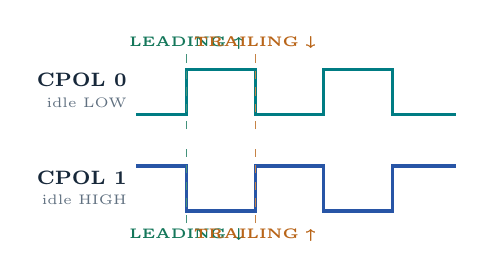
\begin{tikzpicture}[x=.58cm,y=.52cm]
 \node[anchor=east,text=ink,font=\bfseries\scriptsize] at (0,2.35){CPOL 0};
 \node[anchor=east,text=muted,font=\tiny] at (0,1.8){idle LOW};
 \draw[cyan,very thick] (0,1.5)--(1.1,1.5)--(1.1,2.6)--(2.6,2.6)--(2.6,1.5)--(4.1,1.5)--(4.1,2.6)--(5.6,2.6)--(5.6,1.5)--(7,1.5);
 \draw[green!80,dashed] (1.1,1.15)--(1.1,3.0); \node[text=green,font=\tiny\bfseries] at (1.1,3.25){LEADING ↑};
 \draw[orange!80,dashed] (2.6,1.15)--(2.6,3.0); \node[text=orange,font=\tiny\bfseries] at (2.6,3.25){TRAILING ↓};

 \node[anchor=east,text=ink,font=\bfseries\scriptsize] at (0,-.05){CPOL 1};
 \node[anchor=east,text=muted,font=\tiny] at (0,-.58){idle HIGH};
 \draw[blue,very thick] (0,.25)--(1.1,.25)--(1.1,-.85)--(2.6,-.85)--(2.6,.25)--(4.1,.25)--(4.1,-.85)--(5.6,-.85)--(5.6,.25)--(7,.25);
 \draw[green!80,dashed] (1.1,-1.15)--(1.1,.65); \node[text=green,font=\tiny\bfseries] at (1.1,-1.45){LEADING ↓};
 \draw[orange!80,dashed] (2.6,-1.15)--(2.6,.65); \node[text=orange,font=\tiny\bfseries] at (2.6,-1.45){TRAILING ↑};
\end{tikzpicture}
\vspace{.35cm}
\begin{center}
\begin{tabular}{c c c}
\toprule
 & \textcolor{green}{\bfseries Leading} & \textcolor{orange}{\bfseries Trailing}\\
\midrule
CPOL 0 & cạnh lên & cạnh xuống\\
CPOL 1 & cạnh xuống & cạnh lên\\
\bottomrule
\end{tabular}
\end{center}
\end{columns}
\vfill
\source{\href{https://www.analog.com/en/resources/analog-dialogue/articles/introduction-to-spi-interface.html}{Analog Devices — Clock polarity and phase}.}
\end{frame}

% ========================= 13 =========================
\begin{frame}[shrink=7]{The Four SPI Modes}
\transwipe[direction=0,duration=.35]
\vspace{-.18cm}
\begin{columns}[T,onlytextwidth]
\column{.57\textwidth}
\renewcommand{\arraystretch}{1.45}
\scriptsize
\begin{tabularx}{\linewidth}{>{\bfseries}c c c c >{\color{green}\bfseries\centering\arraybackslash}X >{\color{orange}\centering\arraybackslash}X}
\toprule
Mode & CPOL & CPHA & Idle & Sample & Shift\\
\midrule
\textcolor{cyan}{0} & 0 & 0 & LOW & ↑ & ↓\\
1 & 0 & 1 & LOW & ↓ & ↑\\
2 & 1 & 0 & HIGH & ↓ & ↑\\
\textcolor{cyan}{3} & 1 & 1 & HIGH & ↑ & ↓\\
\bottomrule
\end{tabularx}
\vspace{.35cm}
\begin{beamercolorbox}[rounded=true,sep=8pt]{block body}
{\color{cyan}\bfseries MẸO NHỚ}\par\vspace{.15cm}
{\small $\mathrm{CPOL}\oplus\mathrm{CPHA}=0$ $\Rightarrow$ sample cạnh \textbf{lên}; bằng 1 $\Rightarrow$ sample cạnh \textbf{xuống}.}
\end{beamercolorbox}
\vspace{.25cm}
{\small\color{muted}Mode 0 và Mode 3 thường gặp; cả hai lấy mẫu cạnh lên nhưng khác mức idle và thời điểm bit đầu xuất hiện.}

\column{.39\textwidth}
{\color{muted}\scriptsize 2 BIT CẤU HÌNH → 4 MODE}\par\vspace{.22cm}
\begin{tikzpicture}[x=.52cm,y=.52cm]
 \foreach \row/\mode/\idle/\sample in {0/0/LOW/↑,1/1/LOW/↓,2/2/HIGH/↓,3/3/HIGH/↑}{
   \node[smallchip,minimum width=1.05cm,draw=cyan] at (0,{2.4-1.25*\row}) {M\mode};
   \node[anchor=west,text=muted,font=\scriptsize] at (1.2,{2.4-1.25*\row}) {idle \idle};
   \node[anchor=west,text=green,font=\bfseries\scriptsize] at (4.2,{2.4-1.25*\row}) {sample \sample};
 }
 \draw[cyan!35,thick] (-1,-1.95) rectangle (7.15,3.05);
 \node[note,text width=3.55cm,minimum width=3.9cm] at (3.05,-2.75) {Tên mode có thể khác giữa datasheet — hãy đối chiếu \textbf{waveform}.};
\end{tikzpicture}
\end{columns}
\vfill
\source{\href{https://www.analog.com/en/resources/analog-dialogue/articles/introduction-to-spi-interface.html}{Analog Devices — Four SPI modes}.}
\end{frame}

% ========================= 14 =========================
\begin{frame}{SPI Timing Diagrams}
\transfade[duration=.35]
\vspace{-.2cm}
\begin{columns}[T,onlytextwidth]
\column{.49\textwidth}
\pill{cyan}{MODE 0 · CPOL 0 · CPHA 0}\par\vspace{.18cm}
{\small\color{muted}Idle LOW · bit đầu hợp lệ trước cạnh lên đầu tiên}\par\vspace{.12cm}
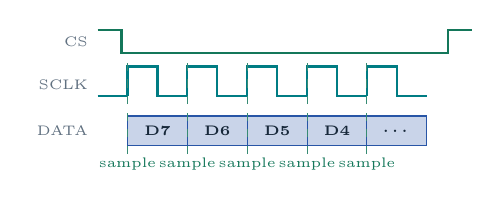
\begin{tikzpicture}[x=.38cm,y=.42cm]
 \node[anchor=east,text=muted,font=\tiny] at (0,3.35){CS};
 \draw[green,thick] (0,3.7)--(.8,3.7)--(.8,3.0)--(11.7,3.0)--(11.7,3.7)--(12.5,3.7);
 \node[anchor=east,text=muted,font=\tiny] at (0,2.05){SCLK};
 \draw[cyan,thick] (0,1.7)--(1,1.7);
 \foreach \x in {1,3,5,7,9}{\draw[cyan,thick] (\x,1.7)--(\x,2.6)--(\x+1,2.6)--(\x+1,1.7)--(\x+2,1.7);}
 \node[anchor=east,text=muted,font=\tiny] at (0,.65){DATA};
 \foreach \x/\v in {1/D7,3/D6,5/D5,7/D4,9/…}{\fill[blue!25] (\x,.2) rectangle ++(2,.9);\draw[blue] (\x,.2) rectangle ++(2,.9);\node[text=ink,font=\tiny\bfseries] at (\x+1,.65){\v};}
 \foreach \x in {1,3,5,7,9}{\draw[green!85,dashed] (\x,-.05)--(\x,2.85);\node[text=green,font=\tiny] at (\x,-.35){sample};}
\end{tikzpicture}
\vspace{.28cm}
\begin{beamercolorbox}[rounded=true,sep=6pt]{block body}
{\scriptsize Cạnh \textcolor{green}{\bfseries lên} lấy mẫu; cạnh \textcolor{orange}{\bfseries xuống} đổi bit.}
\end{beamercolorbox}

\column{.49\textwidth}
\pill{orange}{MODE 3 · CPOL 1 · CPHA 1}\par\vspace{.18cm}
{\small\color{muted}Idle HIGH · bit đầu xuất hiện ở cạnh xuống đầu tiên}\par\vspace{.12cm}
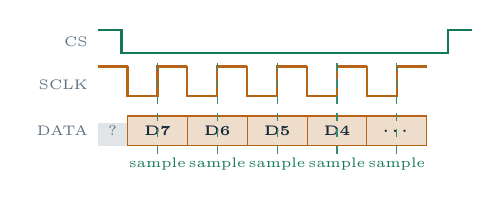
\begin{tikzpicture}[x=.38cm,y=.42cm]
 \node[anchor=east,text=muted,font=\tiny] at (0,3.35){CS};
 \draw[green,thick] (0,3.7)--(.8,3.7)--(.8,3.0)--(11.7,3.0)--(11.7,3.7)--(12.5,3.7);
 \node[anchor=east,text=muted,font=\tiny] at (0,2.05){SCLK};
 \draw[orange,thick] (0,2.6)--(1,2.6);
 \foreach \x in {1,3,5,7,9}{\draw[orange,thick] (\x,2.6)--(\x,1.7)--(\x+1,1.7)--(\x+1,2.6)--(\x+2,2.6);}
 \node[anchor=east,text=muted,font=\tiny] at (0,.65){DATA};
 \fill[muted!18] (0,.2) rectangle (1,.9); \node[text=muted,font=\tiny] at (.5,.65){?};
 \foreach \x/\v in {1/D7,3/D6,5/D5,7/D4,9/…}{\fill[orange!22] (\x,.2) rectangle ++(2,.9);\draw[orange] (\x,.2) rectangle ++(2,.9);\node[text=ink,font=\tiny\bfseries] at (\x+1,.65){\v};}
 \foreach \x in {2,4,6,8,10}{\draw[green!85,dashed] (\x,-.05)--(\x,2.85);\node[text=green,font=\tiny] at (\x,-.35){sample};}
\end{tikzpicture}
\vspace{.28cm}
\begin{beamercolorbox}[rounded=true,sep=6pt]{block body}
{\scriptsize Cạnh \textcolor{green}{\bfseries lên} lấy mẫu; leading edge là cạnh \textcolor{orange}{\bfseries xuống}.}
\end{beamercolorbox}
\end{columns}
\vfill
\source{Waveform khái niệm; cấu hình thực tế phải theo timing diagram của peripheral.}
\end{frame}

% ========================= 15 =========================
\begin{frame}[shrink=10]{Timing Constraints}
\transwipe[direction=90,duration=.35]
\vspace{-.18cm}
\begin{columns}[T,onlytextwidth]
\column{.54\textwidth}
{\color{cyan}\bfseries DATA PHẢI ỔN ĐỊNH QUANH CẠNH LẤY MẪU}\par\vspace{.2cm}
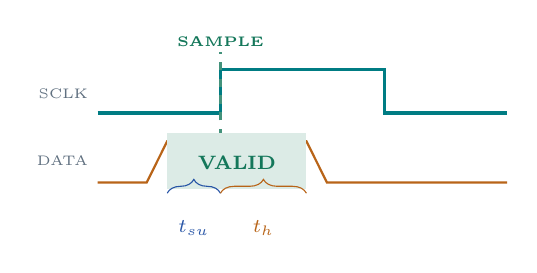
\begin{tikzpicture}[x=.52cm,y=.55cm]
 \node[anchor=east,text=muted,font=\tiny] at (0,2.25){SCLK};
 \draw[cyan,very thick] (0,1.8)--(3,1.8)--(3,2.8)--(7,2.8)--(7,1.8)--(10,1.8);
 \draw[green!80,dashed,thick] (3,.1)--(3,3.2); \node[text=green,font=\tiny\bfseries] at (3,3.45){SAMPLE};
 \node[anchor=east,text=muted,font=\tiny] at (0,.7){DATA};
 \draw[orange,thick] (0,.2)--(1.2,.2)--(1.7,1.15)--(5.1,1.15)--(5.6,.2)--(10,.2);
 \fill[green!15] (1.7,.05) rectangle (5.1,1.35);
 \draw[decorate,decoration={brace,amplitude=5pt},blue] (1.7,-.05)--(3,-.05) node[midway,below=.22cm,text=blue,font=\scriptsize\bfseries]{$t_{su}$};
 \draw[decorate,decoration={brace,amplitude=5pt},orange] (3,-.05)--(5.1,-.05) node[midway,below=.22cm,text=orange,font=\scriptsize\bfseries]{$t_h$};
 \node[text=green,font=\scriptsize\bfseries] at (3.4,.65){VALID};
\end{tikzpicture}
\vspace{.35cm}
\scriptsize
\begin{tabularx}{\linewidth}{>{\color{cyan}\bfseries}l X}
$t_{su}$ / $t_h$ & Setup trước / hold sau cạnh sample\\
$t_{CO}$ & Clock đến lúc MISO hợp lệ\\
CS setup/hold & Khoảng bảo vệ trước xung đầu / sau xung cuối\\
$t_{HIGH}/t_{LOW}$ & Độ rộng tối thiểu hai nửa chu kỳ\\
\end{tabularx}

\column{.42\textwidth}
\begin{beamercolorbox}[rounded=true,sep=8pt]{block body}
{\color{orange}\bfseries TIMING BUDGET · MISO}\par\vspace{.3cm}
{\small\centering $\displaystyle \frac{T_{SCLK}}{2}\ge t_{pd,clk}+t_{CO}+t_{pd,data}+t_{su}$\par}
\end{beamercolorbox}
\vspace{.28cm}
{\small\color{muted}Ví dụ \textbf{giả định}:}\par\vspace{.12cm}
\begin{align*}
t_{CO}&=15\,ns,\quad t_{su}=5\,ns\\
t_{pd,clk}&=t_{pd,data}=1\,ns\\[-2pt]
T/2&\ge22\,ns\Rightarrow T\ge44\,ns
\end{align*}
\begin{center}\metric{orange}{$f_{SCLK}\le22.7$ MHz}{giới hạn từ ví dụ giả định}\end{center}
\vspace{.15cm}
\begin{beamercolorbox}[rounded=true,sep=6pt]{block body}
{\scriptsize Sai mode hoặc thiếu setup/hold $\Rightarrow$ lấy mẫu đúng lúc dữ liệu đang đổi $\Rightarrow$ lệch bit.}
\end{beamercolorbox}
\end{columns}
\vfill
\source{Mô hình timing đơn giản hóa; kiểm tra các giá trị thật trong datasheet của cả controller và peripheral.}
\end{frame}

% ========================= 16 =========================
\begin{frame}[shrink=14]{Clock Frequency \& Data Throughput}
\transfade[duration=.35]
\vspace{-.2cm}
\begin{columns}[T,onlytextwidth]
\column{.42\textwidth}
\begin{beamercolorbox}[rounded=true,sep=9pt]{block body}
{\color{cyan}\bfseries RAW THROUGHPUT}\par\vspace{.3cm}
{\small Bit rate $=f_{SCLK}$}\par
{\small Byte rate $=f_{SCLK}/8$}\par
{\small $t_N=8N/f_{SCLK}$}
\end{beamercolorbox}
\vspace{.25cm}
\begin{center}\metric{cyan}{10 Mbit/s}{10 MHz SCLK}\hspace{.2cm}\metric{green}{1.25 MB/s}{byte rate thô}\end{center}
\vspace{.3cm}
{\color{orange}\bfseries OVERHEAD}\par\vspace{.15cm}
{\small\color{muted}Command + address + dummy + CS timing + khoảng trống phần mềm.}
\vspace{.25cm}
\begin{beamercolorbox}[rounded=true,sep=7pt]{block body}
{\scriptsize Ví dụ flash: \textbf{4 byte overhead}, $f_{SCLK}=10$ MHz — toàn bộ số liệu bên phải là \textbf{giả định minh họa}.}
\end{beamercolorbox}

\column{.54\textwidth}
{\color{muted}\scriptsize HIỆU SUẤT PAYLOAD / TỔNG BYTE TRÊN BUS}\par\vspace{.28cm}
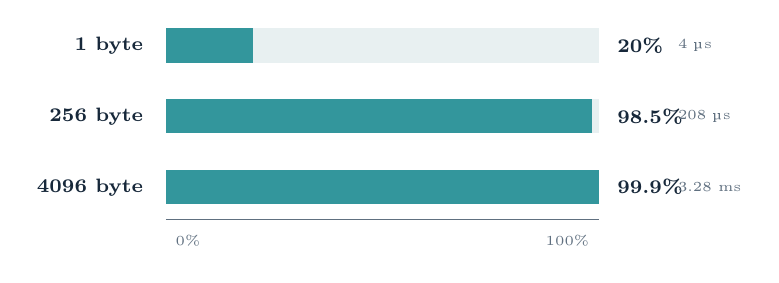
\begin{tikzpicture}[x=.055cm,y=.9cm]
 \foreach \y/\label/\val/\time in {3/1 byte/20/4 µs,2/256 byte/98.5/208 µs,1/4096 byte/99.9/3.28 ms}{
   \node[anchor=east,text=ink,font=\scriptsize\bfseries] at (-3,\y){\label};
   \fill[paneltwo] (0,\y-.24) rectangle (100,\y+.24);
   \fill[cyan!80] (0,\y-.24) rectangle (\val,\y+.24);
   \node[anchor=west,text=ink,font=\scriptsize\bfseries] at (102,\y){\val\%};
   \node[anchor=west,text=muted,font=\tiny] at (116,\y){\time};
 }
 \draw[muted,thin] (0,.55)--(100,.55);
 \node[anchor=west,text=muted,font=\tiny] at (0,.25){0\%}; \node[anchor=east,text=muted,font=\tiny] at (100,.25){100\%};
\end{tikzpicture}
\vspace{.3cm}
\begin{beamercolorbox}[rounded=true,sep=8pt]{block body}
{\color{orange}\bfseries KHOẢNG TRỐNG PHẦN MỀM}\par\vspace{.18cm}
{\small 256 B: $208\,\mu s + 260\times1\,\mu s=468\,\mu s$}\par\vspace{.1cm}
\pill{orange}{1.23 MB/s → 0.55 MB/s}
\end{beamercolorbox}
\vspace{.28cm}
{\small\textcolor{green}{\bfseries Kết luận:} burst càng dài, tỷ lệ payload càng gần tốc độ thô.}
\end{columns}
\vfill
\source{Các phép tính minh họa từ mô hình 1-bit SPI; không phải số đo trên phần cứng.}
\end{frame}

% ========================= 17 =========================
\begin{frame}[shrink=8]{SPI Electrical Characteristics}
\transwipe[direction=0,duration=.35]
\vspace{-.18cm}
\begin{columns}[T,onlytextwidth]
\column{.55\textwidth}
{\color{cyan}\bfseries LOGIC LEVEL ≠ “CHỈ CẦN NỐI DÂY”}\par\vspace{.25cm}

\begin{tikzpicture}[x=1cm,y=1cm]
 \node[device,minimum width=1.9cm,minimum height=2.0cm] (m) at (0,0) {\bfseries MCU\\\color{cyan}\large 3.3 V};
 \node[smallchip,minimum width=1.8cm,minimum height=1.65cm,draw=green] (l) at (3.05,0) {LEVEL\\SHIFTER};
 \node[device,minimum width=1.95cm,minimum height=2.0cm,draw=orange] (p) at (6.1,0) {\bfseries PERIPHERAL\\\color{orange}\large 1.8 V};
 \draw[sig,blue] (m.north east)--node[above,text=blue,font=\tiny\bfseries]{SCLK · MOSI · CS}(l.north west);
 \draw[sig,blue] (l.north east)--(p.north west);
 \draw[sig,orange] (p.south west)--(l.south east);
 \draw[sig,orange] (l.south west)--node[below,text=orange,font=\tiny\bfseries]{MISO}(m.south east);
\end{tikzpicture}
\vspace{.3cm}
\begin{beamercolorbox}[rounded=true,sep=7pt]{block body}
{\small\textbf{VOH/VOL} của bên phát phải nằm ngoài vùng ngưỡng \textbf{VIH/VIL} của bên nhận. Chênh điện áp có thể gây sai logic hoặc hỏng chân.}
\end{beamercolorbox}
\vspace{.3cm}
{\small Ví dụ CMOS tham khảo ở $V_{DD}=3.3$ V:}\par\vspace{.12cm}
\pill{green}{$V_{IH}\approx2.31$ V}\hspace{.3em}\pill{orange}{$V_{IL}\approx0.99$ V}

\column{.41\textwidth}
\begin{beamercolorbox}[rounded=true,sep=8pt]{block body}
{\color{cyan}\bfseries CHECKLIST ĐIỆN}\par\vspace{.22cm}
\begin{itemize}\small
 \item GND chung, đường hồi ngắn.
 \item MISO high-Z khi không được chọn.
 \item SCLK/MOSI/MISO là \textbf{push-pull}; không cần pull-up như I²C.
 \item Pull-up cho CS để tránh chọn nhầm lúc MCU reset.
 \item Kiểm tra absolute maximum rating trước khi nối khác mức.
\end{itemize}
\end{beamercolorbox}
\vspace{.35cm}
\begin{tikzpicture}[x=.7cm,y=.55cm]
 \fill[red!20] (0,2) rectangle (5,2.7); \node[text=red,font=\scriptsize\bfseries] at (2.5,2.35){HIGH · ≥ VIH};
 \fill[muted!15] (0,.9) rectangle (5,2); \node[text=muted,font=\scriptsize] at (2.5,1.45){UNDEFINED};
 \fill[green!20] (0,.2) rectangle (5,.9); \node[text=green,font=\scriptsize\bfseries] at (2.5,.55){LOW · ≤ VIL};
\end{tikzpicture}
\end{columns}
\vfill
\source{Ngưỡng 0.7/0.3 $V_{DD}$ chỉ là ví dụ CMOS; luôn dùng thông số của datasheet.}
\end{frame}

% ========================= 18 =========================
\begin{frame}[shrink=6]{Signal Integrity \& PCB Design}
\transfade[duration=.35]
\vspace{-.2cm}
\begin{columns}[T,onlytextwidth]
\column{.45\textwidth}
{\color{cyan}\bfseries SCLK LÝ TƯỞNG}\par\vspace{.15cm}

\begin{tikzpicture}[x=.52cm,y=.5cm]
 \draw[cyan,very thick] (0,0)--(1,0)--(1,1.3)--(3,1.3)--(3,0)--(5,0)--(5,1.3)--(7,1.3);
\end{tikzpicture}
\vspace{.22cm}
{\color{orange}\bfseries SCLK CÓ RINGING}\par\vspace{.15cm}
\begin{tikzpicture}[x=.52cm,y=.5cm]
 \draw[orange,very thick] plot[smooth] coordinates {(0,0)(1,0)(1.05,1.7)(1.2,.9)(1.4,1.55)(1.7,1.18)(2.1,1.35)(3,1.3)(3.05,-.45)(3.2,.35)(3.45,-.2)(3.8,.08)(5,0)(5.05,1.7)(5.2,.9)(5.5,1.45)(6,1.28)(7,1.3)};
 \draw[red,dashed] (0,.75)--(7,.75); \node[anchor=west,text=red,font=\tiny] at (7.1,.75){threshold};
 \node[note,text width=3.8cm,minimum width=4.1cm] at (3.5,-1.05) {Ringing vượt threshold có thể tạo \textbf{cạnh clock giả}.};
\end{tikzpicture}
\vspace{.25cm}
\begin{beamercolorbox}[rounded=true,sep=7pt]{block body}
{\scriptsize Quy tắc kinh nghiệm: nếu propagation delay $>t_r/6$, hãy xem trace là đường truyền. Với $t_r=2$ ns, khoảng 5 cm đã đáng chú ý (\textbf{giả định}).}
\end{beamercolorbox}

\column{.51\textwidth}
{\color{cyan}\bfseries 5 QUY TẮC PCB}\par\vspace{.2cm}
\begin{tikzpicture}[node distance=.17cm]
 \node[smallchip,minimum width=6.0cm,anchor=west,draw=cyan] (a) at (0,0) {1 · Trace ngắn; cân bằng SCLK / data};
 \node[smallchip,minimum width=6.0cm,anchor=west,draw=orange,below=of a] (b) {2 · Series 22–47 Ω sát driver (tham khảo)};
 \node[smallchip,minimum width=6.0cm,anchor=west,draw=blue,below=of b] (c) {3 · Tránh song song dài; tăng khoảng cách};
 \node[smallchip,minimum width=6.0cm,anchor=west,draw=green,below=of c] (d) {4 · Ground plane liên tục bên dưới};
 \node[smallchip,minimum width=6.0cm,anchor=west,draw=cyan,below=of d] (e) {5 · Stub ngắn; topology gọn};
\end{tikzpicture}
\vspace{.38cm}
\begin{beamercolorbox}[rounded=true,sep=8pt]{block body}
{\small\textcolor{orange}{\bfseries Breadboard + jumper dài} thường là giới hạn đầu tiên khi tăng SCLK — không phải phần mềm.}
\end{beamercolorbox}
\end{columns}
\vfill
\source{\href{https://www.st.com/resource/en/application_note/an5543-guidelines-for-enhanced-spi-communication-on-stm32-mcus-and-mpus-stmicroelectronics.pdf}{ST AN5543}; giá trị termination phải được xác nhận bằng mô phỏng/đo thực tế.}
\end{frame}

% ========================= 19 =========================
\begin{frame}[shrink=11]{SPI Peripheral Configuration}
\transwipe[direction=90,duration=.35]
\vspace{-.2cm}
\begin{columns}[T,onlytextwidth]
\column{.65\textwidth}
{\color{muted}\scriptsize CHECKLIST KHỞI TẠO CONTROLLER}\par\vspace{.2cm}
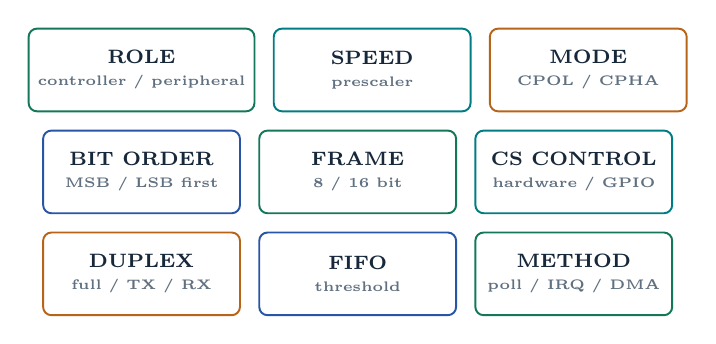
\begin{tikzpicture}[node distance=.22cm and .22cm]
 \node[smallchip,minimum width=2.5cm,minimum height=1.05cm,draw=green] (r) {ROLE\\\color{muted}\tiny controller / peripheral};
 \node[smallchip,minimum width=2.5cm,minimum height=1.05cm,right=of r,draw=cyan] (s) {SPEED\\\color{muted}\tiny prescaler};
 \node[smallchip,minimum width=2.5cm,minimum height=1.05cm,right=of s,draw=orange] (m) {MODE\\\color{muted}\tiny CPOL / CPHA};
 \node[smallchip,minimum width=2.5cm,minimum height=1.05cm,below=of r,draw=blue] (o) {BIT ORDER\\\color{muted}\tiny MSB / LSB first};
 \node[smallchip,minimum width=2.5cm,minimum height=1.05cm,right=of o,draw=green] (f) {FRAME\\\color{muted}\tiny 8 / 16 bit};
 \node[smallchip,minimum width=2.5cm,minimum height=1.05cm,right=of f,draw=cyan] (c) {CS CONTROL\\\color{muted}\tiny hardware / GPIO};
 \node[smallchip,minimum width=2.5cm,minimum height=1.05cm,below=of o,draw=orange] (d) {DUPLEX\\\color{muted}\tiny full / TX / RX};
 \node[smallchip,minimum width=2.5cm,minimum height=1.05cm,right=of d,draw=blue] (q) {FIFO\\\color{muted}\tiny threshold};
 \node[smallchip,minimum width=2.5cm,minimum height=1.05cm,right=of q,draw=green] (mth) {METHOD\\\color{muted}\tiny poll / IRQ / DMA};
\end{tikzpicture}
\vspace{.35cm}
\begin{beamercolorbox}[rounded=true,sep=7pt]{block body}
{\small $f_{SCLK}=f_{PCLK}/\text{prescaler}$ — chọn tốc độ \textbf{không vượt giới hạn chậm nhất} của MCU, peripheral, timing và PCB.}
\end{beamercolorbox}

\column{.31\textwidth}
\begin{beamercolorbox}[rounded=true,sep=8pt]{block body}
{\color{cyan}\bfseries STM32}\par\vspace{.2cm}
{\small CubeMX / HAL: baud prescaler, CPOL, CPHA, first bit, data size, NSS.}
\end{beamercolorbox}
\vspace{.28cm}
\begin{beamercolorbox}[rounded=true,sep=8pt]{block body}
{\color{orange}\bfseries ESP-IDF}\par\vspace{.2cm}
{\small chân bus, \texttt{clock\_speed\_hz}, \texttt{mode}, CS, command/address/dummy, queue.}
\end{beamercolorbox}
\vspace{.3cm}
\begin{beamercolorbox}[rounded=true,sep=7pt]{block body}
{\scriptsize\textcolor{green}{\bfseries Dùng CS GPIO} khi cần giữ CS thấp qua nhiều frame hoặc điều khiển transaction đặc biệt.}
\end{beamercolorbox}
\end{columns}
\vfill
\source{\href{https://docs.espressif.com/projects/esp-idf/en/stable/esp32/api-reference/peripherals/spi_master.html}{Espressif — SPI Master Driver}; cấu hình STM32 phụ thuộc dòng MCU.}
\end{frame}

% ========================= 20 =========================
\begin{frame}[shrink=3]{SPI Programming Methods}
\transfade[duration=.35]
\vspace{-.2cm}
\begin{columns}[T,onlytextwidth]
\column{.67\textwidth}
\begin{tikzpicture}[x=.78cm,y=.8cm]
 \foreach \y/\name/\clr/\desc in {3/POLLING/cyan/CPU đọc cờ liên tục,2/INTERRUPT/orange/CPU chạy ISR theo sự kiện,1/DMA/green/DMA tự chuyển RAM ↔ SPI}{
   \node[smallchip,minimum width=1.8cm,draw=\clr] (n\y) at (0,\y) {\name};
   \node[anchor=west,text=ink,font=\scriptsize] at (1.6,\y+.18){\desc};
   \draw[muted!45,line width=5pt] (1.6,\y-.22)--(8.1,\y-.22);
 }
 % CPU busy timelines
 \draw[cyan,line width=5pt] (1.6,2.78)--(8.1,2.78);
 \foreach \x in {1.8,3.2,4.6,6.0,7.4}{\draw[orange,line width=5pt] (\x,1.78)--(\x+.35,1.78);}
 \draw[green,line width=5pt] (1.6,.78)--(2.0,.78); \draw[green,line width=5pt] (7.7,.78)--(8.1,.78);
 \node[anchor=west,text=muted,font=\tiny] at (8.35,2.78){CPU bận 100\%};
 \node[anchor=west,text=muted,font=\tiny] at (8.35,1.78){bận từng đoạn};
 \node[anchor=west,text=muted,font=\tiny] at (8.35,.78){setup + done};
\end{tikzpicture}
\vspace{.3cm}
\renewcommand{\arraystretch}{1.18}
\setlength{\tabcolsep}{2pt}
\tiny
\begin{tabularx}{\linewidth}{>{\color{muted}\bfseries}l X X X}
\toprule
 & \textcolor{cyan}{Polling} & \textcolor{orange}{Interrupt} & \textcolor{green}{DMA}\\
\midrule
Ưu & đơn giản, latency thấp & CPU rảnh giữa IRQ & CPU gần như rảnh\\
Nhược & chiếm CPU & overhead mỗi IRQ & setup/cache phức tạp\\
Hợp với & vài byte & tải vừa, sự kiện & buffer lớn, liên tục\\
\bottomrule
\end{tabularx}

\column{.29\textwidth}
\begin{beamercolorbox}[rounded=true,sep=8pt]{block body}
{\color{cyan}\bfseries STM32 HAL}\par\vspace{.28cm}
{\scriptsize\ttfamily HAL\_SPI\_TransmitReceive()}\par\vspace{.2cm}
{\scriptsize\ttfamily ...\_IT()}\par\vspace{.2cm}
{\scriptsize\ttfamily ...\_DMA()}
\end{beamercolorbox}
\vspace{.35cm}
\begin{beamercolorbox}[rounded=true,sep=7pt]{block body}
{\small\textcolor{orange}{\bfseries Không có phương pháp luôn tốt nhất.} Điểm chuyển polling → DMA phải đo trên nền tảng thật.}
\end{beamercolorbox}
\end{columns}
\vfill
\source{Tên API minh họa theo STM32 HAL; kiểm tra tài liệu đúng dòng MCU và phiên bản thư viện.}
\end{frame}

% ========================= 21 =========================
\begin{frame}[shrink=2]{Practical SPI Programming}
\transwipe[direction=0,duration=.35]
\vspace{-.2cm}
\begin{columns}[T,onlytextwidth]
\column{.55\textwidth}
{\color{cyan}\bfseries ĐỌC MỘT THANH GHI · POLLING}\par\vspace{.18cm}
\begin{beamercolorbox}[rounded=true,sep=7pt]{block body}
{\ttfamily\scriptsize
spi\_init(mode=0, clock=1MHz, MSB, 8bit);\\[3pt]
function read\_register(addr):\\
\hspace*{1em}tx = [addr | READ\_FLAG, 0x00]\\
\hspace*{1em}\textcolor{green}{cs\_low()}\\
\hspace*{1em}rx = spi\_transfer(tx, length=2)\\
\hspace*{1em}\textcolor{orange}{cs\_high()}\\
\hspace*{1em}return rx[1]
}
\end{beamercolorbox}
\vspace{.25cm}
\begin{beamercolorbox}[rounded=true,sep=7pt]{block body}
{\ttfamily\tiny
uint8\_t tx[2] = \{0x8F, 0x00\}; // minh họa\\
uint8\_t rx[2];\\[2pt]
HAL\_GPIO\_WritePin(CS, RESET);\\
HAL\_SPI\_TransmitReceive(\&hspi1, tx, rx, 2, 100);\\
HAL\_GPIO\_WritePin(CS, SET);\\
uint8\_t value = rx[1];
}
\end{beamercolorbox}

\column{.41\textwidth}
{\color{muted}\scriptsize TRANSACTION TƯƠNG ỨNG}\par\vspace{.2cm}
\begin{tikzpicture}[x=.63cm,y=.55cm]
 \node[anchor=east,text=muted,font=\tiny] at (0,2.2){CS};
 \draw[green,thick] (0,2.55)--(.6,2.55)--(.6,1.75)--(7.4,1.75)--(7.4,2.55)--(8,2.55);
 \fill[blue!45] (.6,.55) rectangle (4,1.45); \node[text=ink,font=\scriptsize\bfseries] at (2.3,1){0x8F · READ};
 \fill[orange!45] (4,.55) rectangle (7.4,1.45); \node[text=ink,font=\scriptsize\bfseries] at (5.7,1){0x00 · DUMMY};
 \draw[orange,very thick,-Latex] (4,.15)--node[below,text=orange,font=\tiny\bfseries]{MISO trả rx[1]}(7.4,.15);
\end{tikzpicture}
\vspace{.3cm}
\begin{beamercolorbox}[rounded=true,sep=8pt]{block body}
{\small Byte nhận đồng thời lúc gửi command thường bỏ qua; \textbf{byte thứ hai} mới là giá trị thanh ghi.}
\end{beamercolorbox}
\vspace{.28cm}
\begin{beamercolorbox}[rounded=true,sep=7pt]{block body}
{\scriptsize\textcolor{orange}{\bfseries Lưu ý:} \texttt{0x8F}, READ\_FLAG, số dummy byte và vị trí dữ liệu đều phụ thuộc datasheet. ESP-IDF biểu diễn cùng thao tác bằng một \texttt{spi\_transaction\_t}.}
\end{beamercolorbox}
\end{columns}
\vfill
\source{\href{https://docs.espressif.com/projects/esp-idf/en/stable/esp32/api-reference/peripherals/spi_master.html}{ESP-IDF SPI Master}; code là cấu trúc minh họa, chưa phải kết quả đo phần cứng.}
\end{frame}

% ========================= 22 =========================
\begin{frame}[shrink=13]{Performance Optimization}
\transfade[duration=.4]
\vspace{-.2cm}
\begin{columns}[T,onlytextwidth]
\column{.47\textwidth}
{\color{cyan}\bfseries 4 ĐÒN BẨY HIỆU NĂNG}\par\vspace{.2cm}
\begin{tikzpicture}[node distance=.18cm]
 \node[smallchip,minimum width=5.65cm,draw=cyan] (a) {1 · Vài byte: polling · khối lớn: DMA};
 \node[smallchip,minimum width=5.65cm,draw=green,below=of a] (b) {2 · Gộp burst · giữ CS thấp};
 \node[smallchip,minimum width=5.65cm,draw=blue,below=of b] (c) {3 · Buffer + FIFO · giảm số ngắt};
 \node[smallchip,minimum width=5.65cm,draw=orange,below=of c] (d) {4 · Loại khoảng trống phần mềm};
\end{tikzpicture}
\vspace{.28cm}
\begin{beamercolorbox}[rounded=true,sep=7pt]{block body}
{\small 10 MHz $\Rightarrow$ 0.8 $\mu$s/byte. Nếu một IRQ tốn 1–2 $\mu$s (\textbf{giả định}), CPU không thể xử lý ngắt theo từng byte $\Rightarrow$ FIFO/DMA.}
\end{beamercolorbox}
\vspace{.25cm}
\begin{beamercolorbox}[rounded=true,sep=7pt]{block body}
{\color{cyan}\bfseries SPEED CEILING}\par\vspace{.15cm}
{\scriptsize $f_{max}=\min(\text{chip},\ \text{MCU/pad},\ \text{timing margin},\ \text{signal integrity})$}
\end{beamercolorbox}

\column{.49\textwidth}
{\color{orange}\bfseries DMA COMPLETE ≠ BUS IDLE}\par\vspace{.18cm}
\begin{tikzpicture}[x=.65cm,y=.62cm]
 \node[anchor=east,text=muted,font=\tiny] at (0,2.5){DMA};
 \draw[green,very thick] (0,2.2)--(4.1,2.2); \draw[muted!45,very thick] (4.1,2.2)--(8,2.2);
 \node[text=green,font=\tiny\bfseries] at (4.1,2.7){COMPLETE};
 \draw[green!80,dashed] (4.1,-.1)--(4.1,3);
 \node[anchor=east,text=muted,font=\tiny] at (0,1.25){SPI BUSY};
 \draw[orange,very thick] (0,.95)--(6.3,.95); \draw[muted!45,very thick] (6.3,.95)--(8,.95);
 \node[text=orange,font=\tiny\bfseries] at (6.3,1.45){BUSY = 0};
 \draw[orange!80,dashed] (6.3,-.1)--(6.3,1.75);
 \node[anchor=east,text=muted,font=\tiny] at (0,.1){CS};
 \draw[cyan,very thick] (0,.35)--(7.2,.35)--(7.2,-.35)--(8,-.35);
 \draw[red,very thick,-Latex] (4.1,-.65)--(4.1,.15); \node[text=red,font=\tiny\bfseries,align=center] at (4.1,-1.05){CS↑ ở đây\\cắt bit cuối};
 \draw[green,very thick,-Latex] (6.3,-.65)--(6.3,.15); \node[text=green,font=\tiny\bfseries,align=center] at (6.3,-1.05){đợi BUSY=0\\rồi CS↑};
\end{tikzpicture}
\vspace{.3cm}
\begin{beamercolorbox}[rounded=true,sep=8pt]{block body}
{\small DMA chỉ báo RAM đã chuyển dữ liệu vào SPI; shift register có thể vẫn đang phát bit cuối.}
\end{beamercolorbox}
\vspace{.25cm}
\pill{cyan}{TIẾP THEO: APPLICATIONS · DEBUG · CASE STUDIES}
\end{columns}
\vfill
\source{Ngưỡng chuyển DMA và chi phí IRQ phụ thuộc nền tảng; phải benchmark và kiểm tra cờ BUSY theo reference manual.}
\end{frame}

\end{document}
